\subsection{Configuración de \gls{term:grafana}}
\label{configuracion-de-grafana}

Como hemos mencionado anteriormente, hemos elegido \gls{term:grafana} para la
creación de los tableros que mostraran la información que hemos recolectado en
el \autoref{cap4}. Para elegir los gráficos incluidos en los tableros es
importante tener en cuenta las necesidades de cada tipo de usuario.

Es posible instalar \gls{term:grafana} en Debian o Ubuntu
\footnote{Sistemas operativos construidos sobre el kernel de \gls{term:linux}},
ejecutando los siguientes comandos en una consola:

\begin{lstlisting}
$ wget https://grafanarel.s3.amazonaws.com/builds/grafana_4.1.2-1486989747_amd64.deb
$ sudo apt-get install -y adduser libfontconfig
$ sudo dpkg -i grafana_4.1.2-1486989747_amd64.deb
\end{lstlisting}

Para iniciar el servicio de \gls{term:grafana} en \gls{term:linux}, basta con
ejecutar el siguiente comando en la terminal:

\begin{lstlisting}
$ sudo service grafana-server start
\end{lstlisting}


Esta orden inicializa el proceso \texttt{grafana-sever} como el usuario
\gls{term:grafana}, que fue creado durante la instalación.

Una vez que el proceso está en ejecución es posible acceder al servicio en el
puerto 3000 del navegador e iniciar sesión.
\footnote{Más información sobre el proceso de instalación de Grafana en \url{http://docs.grafana.org/}}

\gls{term:grafana} soporta varios \eng{backends} de almacenamiento diferentes,
llamados \glspl{term:datasource}. Cada uno de ellos tiene un editor de consultas
visual específico, para facilitar el armado de paneles de control a los
usuarios.

\gls{term:grafana} tiene soporte para tomar información de las siguientes bases
de datos, herramientas y servicios:

\begin{itemize}
  \item CloudWatch
  \item \gls{term:elasticsearch}
  \item Graphite
  \item \gls{term:influx}
  \item KairosDB
  \item OpenTSDB
  \item Prometheus
\end{itemize}

Para conectar \gls{term:grafana} con la instancia de \gls{term:influx}
configurada en el capítulo anterior, se debe comenzar por crear un \gls{term:datasource}
que consuma información de la base de datos.

\begin{figure}
  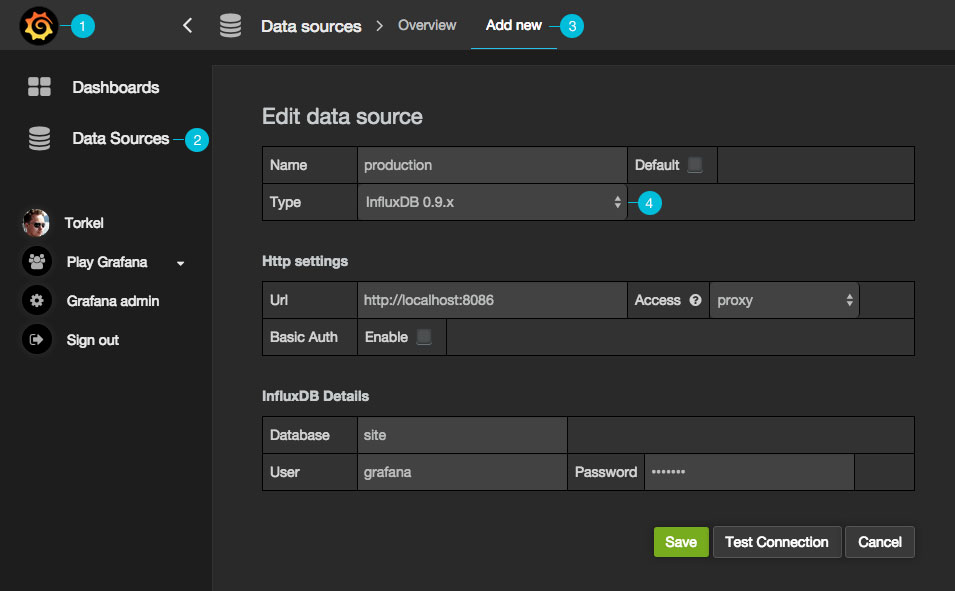
\includegraphics[width=\linewidth]{src/images/05-capitulo-5/datasource-grafana.jpg}
  \caption{Cómo configurar un \gls{term:datasource} para tomar datos de \gls{term:influx}}
  \label{fig:datasource-grafana}
\end{figure}

En la \autoref{fig:datasource-grafana} se pueden ver los pasos para crear un
\gls{term:datasource} en el cliente \eng{web} de \gls{term:grafana}. Los pasos son los
siguientes:

\begin{enumerate}
  \item Abrir el menú haciendo click en el ícono de \gls{term:grafana} en el
  navegador ubicado en la parte superior de la página.

  \item Una vez abierto el menú, hacer click en el enlace \texttt{DataSources}.
  \item Hacer click en el botón \texttt{Add new link} en el navegador.
  \item Llenar el formulario con los datos:
    \begin{itemize}
      \item \textbf{Name:}
      El nombre del \gls{term:datasource}.

      \item \textbf{Default:}
      Si este campo es activado, el \gls{term:datasource} será preseleccionado
      para nuevos paneles.

      \item \textbf{Url:}
      El protocolo \gls{acro:http}, \gls{acro:ip} y puerto de la \gls{term:api}
      \gls{term:influx}

      \item \textbf{Access:}
      Si se selecciona \texttt{Proxy} , se accede a través del backend de \gls{term:grafana}.
      Si se selecciona \texttt{Direct}, se accede directamente desde el navegador.

      \item \textbf{Database:}
      Nombre de la base de datos de \gls{term:influx}

      \item \textbf{User:}
      Nombre del usuario de la base de datos.

      \item \textbf{Password:}
      Contraseña del usuario de la base de datos.

    \end{itemize}
\end{enumerate}

Una vez creado nuestro \gls{term:datasource} podemos comenzar a crear tableros
en \gls{term:grafana}.

Por ejemplo, a partir de los datos almacenados en \gls{term:influx}, podemos
crear gráficos con la intención de que sean útiles a un responsable de IT de la
aplicación. En dichos gráficos podemos elegir que se visualice el tiempo de
respuesta de la aplicación, el rendimiento de sus componentes, disponibilidad
total de la aplicación, cantidad de espacio en disco y memoria usada por el
servidor.

Si quisiéramos medir el tiempo de respuesta de la aplicación \gls{term:ror},
podríamos optar por un gráfico de líneas donde el eje horizontal sea la hora, y
el eje vertical sea el tiempo de respuesta. Dicho gráfico podría aprovechar la
información que hemos enviado desde la aplicación \gls{term:ror} a
\gls{term:influx} en la \autoref{configuracion_de_las_aplicaciones}. El gráfico
se encontraría desglosado en tiempo de renderizado de las vistas, tiempo de
acceso a las bases de datos, y otros tiempos, y se vería como el siguiente:

Para poder recrear dicho gráfico hemos debido realizar varias consultas a la
base de datos \gls{term:influx} configurada en el capítulo anterior usando la
herramienta visual provista por \gls{term:grafana}.

A modo de ejemplo, mostraremos cómo podemos usar grafana para medir la
experiencia de usuario utilizando la métrica Apdex.

Apdex es un método estándar para reportar y comparar el rendimiento de
aplicaciones de software. Su propósito es convertir medidas en información
sobre la satisfacción del usuario especificando una forma uniforme de analizar
y reportar el grado en el que el rendimiento medido cumple las expectativas del
usuario.

Hemos estudiado diferentes maneras de mostrar esta información y consensuamos
en utilizar un gráfico de barras donde cada barra se corresponda con un período
de 1 hora, con el objetivo de contemplar la variación del valor apdex en las
anteriores 24 horas. De esta forma podemos analizar si influyen de algún modo
las franjas horarias en la experiencia final del usuario.

En este capítulo hemos mostrado cómo se pueden configurar algunas herramientas
de visualización para reflejar los datos que hemos almacenado hasta ahora en
\gls{term:influx} y en \gls{term:elasticsearch}. En el capítulo siguiente
mostraremos cómo crear alertas que permitan a los usuarios descubrir de forma
rápida eventos a los que deberían prestar atención.
